\subsection{Comparison with Soft Actor-Critic}
\label{subsec:sac_comparison}

To assess the dependence of the results on the learning algorithm, soft actor-critic (SAC)~\cite{haarnoja2018soft} is evaluated on the same single-input Node 2 and Node 3 tasks. Both algorithms use the six-dimensional observation $(\mathbf x,\mathbf e)/5$, reward $-0.1\|\mathbf e\|_1$, actuator bound $|u|\leq4$, nominal training dynamics, and final checkpoints at a nominal budget of $4\times10^5$ environment transitions. Three independent training runs and 20 common test initial conditions per seed are used. All checkpoints are retained, and evaluation uses deterministic actions without online learning. The compared test settings are nominal dynamics, mismatch $\eta=2$, the drive-state impulse at $t=10$, and response process noise with $\sigma=0.05$.

Both implementations use two hidden layers of width 64, a learning rate of $3\times10^{-4}$, batch size 128, and discount factor 0.99. PPO uses Tanh hidden activations, four environments with 512 steps per rollout, ten optimization epochs, clip range 0.2, GAE parameter 0.95, and entropy coefficient 0.001. SAC uses ReLU hidden activations, one environment, a replay buffer of $10^5$ transitions, 5,000 initial exploration steps, one gradient update per subsequent transition, target-update coefficient $\tau=0.005$, and automatic entropy adjustment with target entropy $-1$. These settings are fixed across nodes and seeds. Equal environment-transition budgets do not imply equal gradient-update counts or training times, and this comparison does not exhaust algorithm-specific hyperparameter tuning.

\begin{table*}[pos=!t,width=\textwidth]
\centering\small
\setlength{\tabcolsep}{2pt}
\caption{PPO and SAC at the same nominal budget of $4\times10^5$ environment transitions. Values are mean $\pm$ sample SD across three training-seed means, each obtained from 20 common test initial conditions. $E_{\mathrm{post}}$ is reported only for the impulse scenario.}
\label{tab:sac_comparison}
\begin{tabular}{@{}cllccc@{}}
\toprule
Node & Scenario & Method & MAE & $E_u$ & $E_{\mathrm{post}}$ \\
\midrule
2 & Nominal & PPO & $0.0930 \pm 0.0022$ & $9.09 \pm 1.53$ & -- \\
2 & Nominal & SAC & $0.1173 \pm 0.0046$ & $6.27 \pm 0.45$ & -- \\
2 & $\eta=2$ & PPO & $0.1703 \pm 0.0085$ & $11.85 \pm 1.60$ & -- \\
2 & $\eta=2$ & SAC & $0.1513 \pm 0.0037$ & $9.31 \pm 0.43$ & -- \\
2 & Impulse & PPO & $0.4339 \pm 0.0246$ & $17.51 \pm 1.19$ & $2.0800 \pm 0.1451$ \\
2 & Impulse & SAC & $0.4206 \pm 0.0979$ & $25.20 \pm 9.79$ & $1.9226 \pm 0.5913$ \\
2 & $\sigma=0.05$ & PPO & $0.2669 \pm 0.0049$ & $135.57 \pm 48.71$ & -- \\
2 & $\sigma=0.05$ & SAC & $0.2632 \pm 0.0052$ & $86.13 \pm 8.86$ & -- \\
\midrule
3 & Nominal & PPO & $0.0431 \pm 0.0012$ & $6.54 \pm 0.34$ & -- \\
3 & Nominal & SAC & $0.0416 \pm 0.0010$ & $4.60 \pm 0.11$ & -- \\
3 & $\eta=2$ & PPO & $0.0656 \pm 0.0025$ & $6.44 \pm 0.30$ & -- \\
3 & $\eta=2$ & SAC & $0.0644 \pm 0.0009$ & $5.07 \pm 0.16$ & -- \\
3 & Impulse & PPO & $0.2581 \pm 0.0003$ & $18.09 \pm 3.50$ & $1.2969 \pm 0.0070$ \\
3 & Impulse & SAC & $0.2735 \pm 0.0106$ & $12.62 \pm 0.53$ & $1.3987 \pm 0.0664$ \\
3 & $\sigma=0.05$ & PPO & $0.1312 \pm 0.0066$ & $69.96 \pm 17.55$ & -- \\
3 & $\sigma=0.05$ & SAC & $0.1273 \pm 0.0013$ & $50.40 \pm 14.21$ & -- \\
\bottomrule
\end{tabular}
\end{table*}


\begin{figure*}[pos=!t,width=\textwidth]
  \centering
  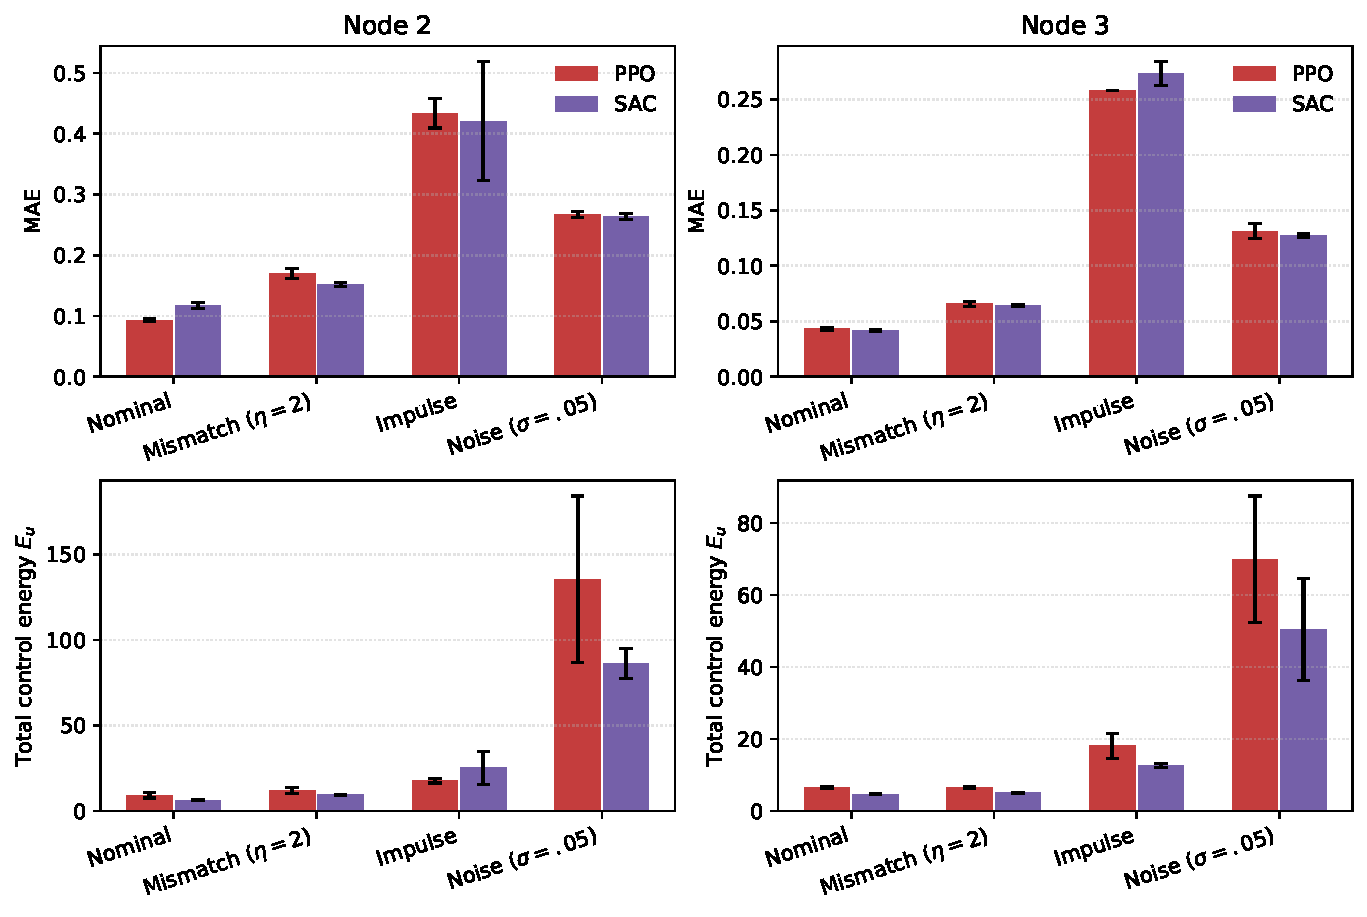
\includegraphics[width=0.78\textwidth]{figures/ppo_sac_matched_budget.pdf}
  \caption{PPO--SAC comparison at matched environment-transition budgets. Bars show the mean of three training-seed means and error bars show their sample standard deviation. Each seed is evaluated on 20 common initial conditions. The upper panels use full-horizon MAE for every scenario; the separate post-impulse metric is given in Table~\ref{tab:sac_comparison}.}
  \label{fig:sac_comparison}
\end{figure*}

Table~\ref{tab:sac_comparison} and Fig.~\ref{fig:sac_comparison} show a scenario-dependent comparison. For Node 2, PPO has lower nominal MAE (0.0930 versus 0.1173), but SAC has lower MAE under mismatch $\eta=2$ (0.1513 versus 0.1703) and also lower energy (9.31 versus 11.85). Following the impulse, SAC has lower mean $E_{\mathrm{post}}$ (1.9226 versus 2.0800), but greater variation across training-seed means (SD 0.5913 versus 0.1451) and higher mean energy (25.20 versus 17.51). At $\sigma=0.05$, the mean MAEs are close (0.2632 for SAC and 0.2669 for PPO), while SAC uses less energy.

For Node 3, SAC has slightly lower mean MAE in the nominal, mismatch, and noise tests and lower mean energy in all four settings. PPO achieves lower post-impulse error (1.2969 versus 1.3987), at higher energy. Thus, the traditional-baseline advantages reported above do not imply that PPO outperforms another learning algorithm in every scenario. PPO is a viable implementation of the constrained pinning framework, while algorithm choice depends on the operating condition and the relative importance of error, variability, and control effort. With only three training seeds, the reported means and SDs are descriptive evidence rather than a general statistical superiority claim.
